The application final design can be analyzed through its abstract deployment diagram:
\begin{figure}[H]
  \centering
  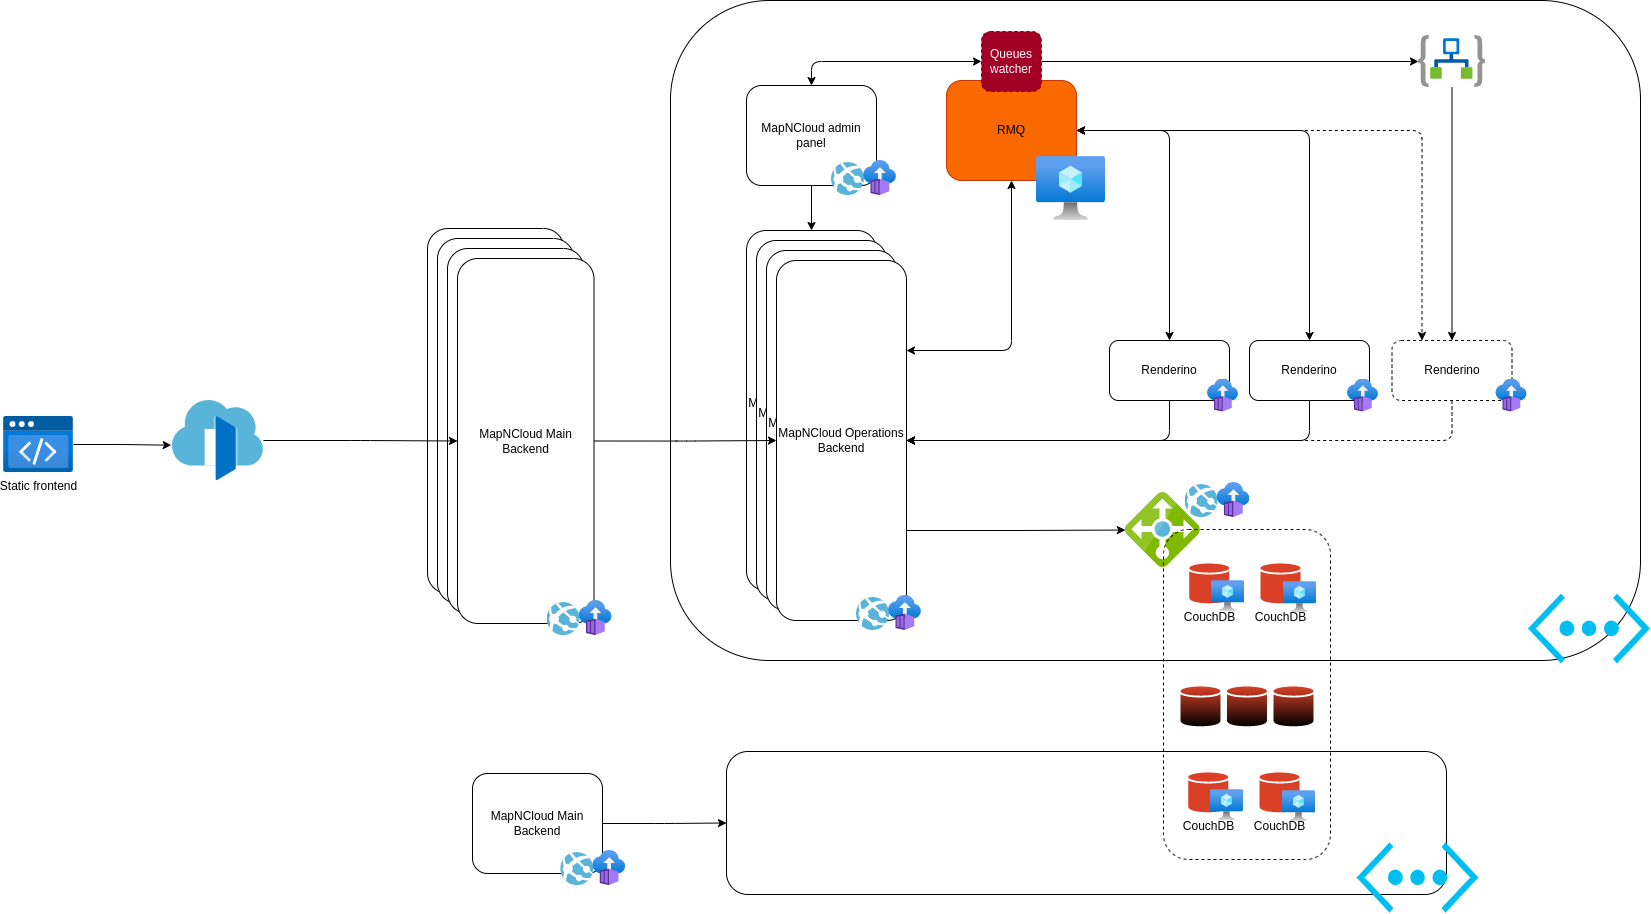
\includegraphics[width = \textwidth]{../Images/SystemDesign-Final.drawio.png}
  \caption{The final MapNCloud architecture}
\end{figure}
While the details of the implementation will be analyzed in further sections, here I would like to give a more high-level vision of the schema.\\
This diagram represents three main aspects of the system: the internal components, their deployment solutions and their "network grouping" which translates then in the geographical organization.

\paragraph{Internal Components}
  The already discussed internal modules can be easily seen in the diagram: the frontend to the far left, the two backend modules in the middle of the diagram, the computational components (with their codename, "Renderino") and the database to the right, the queue managing system and the admin panel on top. In this diagram are represented the "active components" of the architecture, the ones that actively participate in providing the service or the ones that are needed to make the infrastructure work (as the load balancer in front of the database instances).

\paragraph{Deployment Solutions}
  The diagram shows, alongside the \textit{active} architecture, the deployment solutions found for each module. As an example, the frontend module is deployed as an Azure Static Web App, which is a simple resource that allows for a code repository to be directly deployed in the cloud. The backends module are deployed either in a Container Instance (the Renderini), which are simple container groups, or Web App for Containers (the backends), which instead are Web Apps complete with CORS and SSL support that can host a container image for the application.\\
  There are many other cloud resources deployed as part of this system; a complete list of all the cloud resources used and their configuration can be found in the design document of the system itself \cite{MNCDesignDoc}.

\paragraph{Geographical Organization}
  The graph also shows two Virtual Networks, which are the bigger blocks that encapsulate most of the architecture. These virtualized addresses spaces serve multiple purposes:
  \begin{itemize}
    \item They isolate the modules from the internet, acting as a private network. Components as the Renderini do not need additional security embedded in the application because of this measure, which "seals off" these modules from the public network.
    \item They enrich the architecture with geographical information: each Virtual Network is deployed in a single geographical region (which is loosely mapped on a data center) and all the resources deployed inside that virtual network must be in the same region. This allows to take into consideration different pools of users: if the user base in another geographical region is growing, the system is designed to be easily replicated in that region. Moreover, the network structure (the internal subnetting organization) takes into account the possible extension to other regions, grouping together databases instances and allowing \textit{subnet peering}\footnote{two peered subnets acts as two connected addresses space in different regions. Since a Cloud Virtual Network can span a single region, subnet peering is a way to extend a protected virtual network to multiple regions}.
    \item They provide an additional layer of organization and grouping on top of the already available one in the cloud resource manager: subnetting. Grouping together homogeneous resources using their network address helps in keeping the structure observable\footnote{from a monitoring perspective}, reachable and easily maintainable and extendable.
  \end{itemize}

\subsection{Containers and Virtual Machines in the final design}
  In the graph is visible how some services (namely RabbitMQ and CouchDB) has been ultimately deployed on Virtual Machines rather then container-oriented resources. This is due to various reasons:
  \begin{itemize}
    \item persistence solution for containers (storage) are not so common in cloud providers, and the only available at writing time are not suited for the deployment of an application, either because of overall performance or cost
    \item some container groups deployed (as the queuing system group) needed to have multiple ports opened and available, which is usually a feature which is not compatible with web components; employing a solution ideal for transients workers as a permanent solution for RabbitMQ (with a much higher cost and much less support or features) would not be the best solution
  \end{itemize}
  However, container technology is used on the virtual machines: the software instances are distributed, installed and run through a container engine. This has multiple benefits: other than the already mentioned simplified management of the package, the configuration and the dependencies, it allow us to abstract from the virtual machine internal configuration. Each one is configured to execute a full system upgrade on startup (or reboot) that could potentially break some dependency if the software would be installed on the machine; being instead pulled alongside all its dependencies, this problem does not exist.
